
\chapter{Introduction}
\label{cha:introduction}

\epigraph{\textit{Remember that all models are wrong; the practical
    question is how wrong do they have to be to not be
    useful.}}{George Box (1987)}

\section{Motivation}
\label{sec:motivation}

Robotic planning algorithms have been widely successful in computing
feasible and optimal plans, or sequence of decisions, for tasks
involving robots operating in known environments or under known
conditions~\cite{DBLP:books/cu/L2006}. A large part of this success
can be attributed to principled algorithms that effectively
``search'' the space of all plans by exploiting the known
structure in the form of dynamical models to quickly compute the
solution~\cite{choset2005principles}. For example in the field of robot motion planning, there
have been various developments in designing planning algorithms that
exploit forward models to effectively discretize the state space into
a graph and compute a feasible plan using graph search
techniques~\cite{DBLP:books/daglib/0068760}. This enables planning
algorithms to guarantee task 
completeness, which is a requirement on the solution plan to complete
the task, and be efficient in the amount of computational resources
needed to find the solution~\cite{DBLP:journals/arobots/Hauser12}.

However for robots to operate in unstructured environments such as
homes, offices and disaster sites, planning algorithms have to
reason about how to deal with the lack of complete knowledge of the
environment while ensuring task completeness~\cite{DBLP:journals/ai/KaelblingLC98}. To retain their
effectiveness, these planning algorithms will have to utilize partial
knowledge of the environment and the task in the form of simplified
and \textit{inaccurate} dynamical models~\cite{abbeel2006using}.
Naively using these inaccurate dynamical models for planning
can result in highly suboptimal plans and in some cases, plans that do
not complete the task during execution~\cite{kolter2010learning}. An example of such behavior is
shown in Figure~\ref{fig:intro-example}. In this example, a robotic arm is
performing a pick-and-place task while avoiding collision with an
obstacle. In the first scenario (the first three figures from the left
in Figure~\ref{fig:intro-example},) the arm is interacting with a
light object whose mass is accurately captured by the dynamical model
used by the planner. This results in a computed trajectory for the
arm that grasps the object, lifts it above the obstacle and takes it
to the goal location. While this scenario has highlighted the
effectiveness of the planning algorithm to complete the task when
given access to an accurate dynamical model, consider the second
scenario (the last figure on the right in
Figure~\ref{fig:intro-example}) where the arm is interacting with a
heavy object which is modeled as a light object by the dynamical
model. Since the model is same as before, the planner computes the
same trajectory which lifts the object above the obstacle. However,
while executing the trajectory the arm cannot lift the heavy object and
cannot command the joint torques required because they are beyond the
arm's capabilities. Thus, the computed plan is not successful in
completing the task.
\begin{figure*}[t]
  \centering
  \begin{subfigure}{0.24\linewidth}
    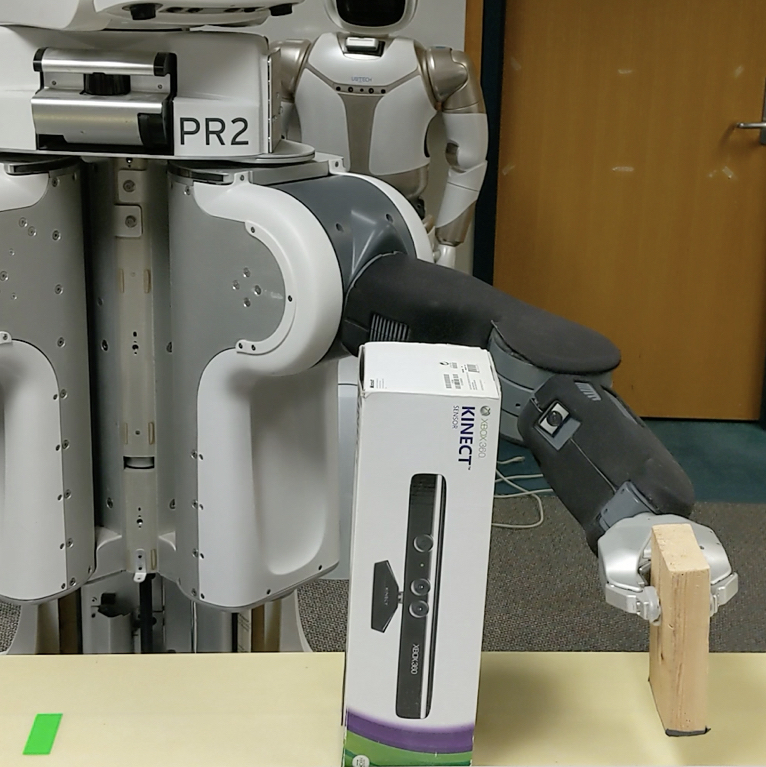
\includegraphics[width=\linewidth]{figures/cmax/pr2_pick_place_light_1_annotated.jpeg}
  \end{subfigure}
  \begin{subfigure}{0.24\linewidth}
    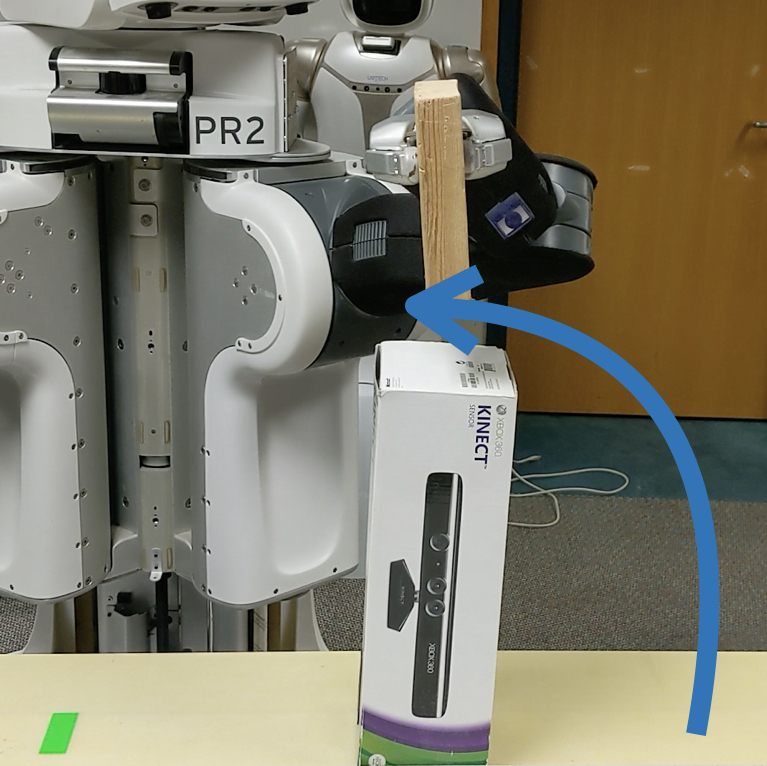
\includegraphics[width=\linewidth]{figures/cmax/pr2_pick_place_light_2_annotated.jpeg}
  \end{subfigure}
  \begin{subfigure}{0.24\linewidth}
    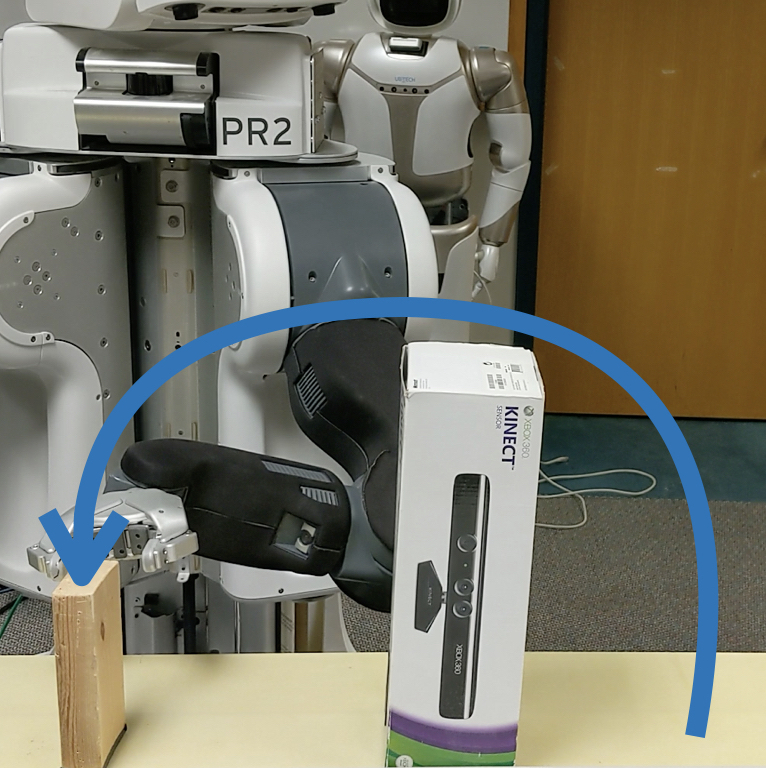
\includegraphics[width=\linewidth]{figures/cmax/pr2_pick_place_light_3_annotated.jpeg}
  \end{subfigure}
  \begin{subfigure}{0.24\linewidth}
    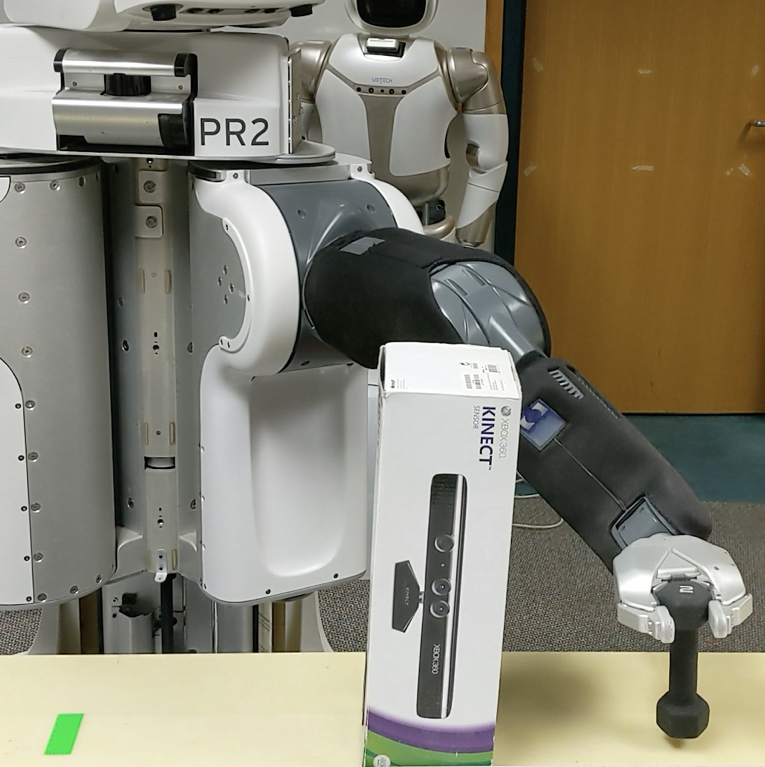
\includegraphics[width=\linewidth]{figures/cmax/pr2_pick_place_heavy_1_annotated.jpeg}
  \end{subfigure}
  \caption{A robotic arm picking an object from its start location and
  placing it at a goal location while avoiding collision with the
  intermediate obstacle during motion. The first three (from left)
  figures show an execution with a light object (wooden block) and a
  plan (blue trajectory) computed
  using an accurate dynamical model which captures the weight of the
  object correctly. The last figure (rightmost) shows an instance of
  the same task but with a heavy object (black dumbbell) and same
  dynamical model as before which models the object as light. This
  results in the planner computing the same plan as before, which the
  robot cannot execute as lifting the heavy object requires joint
  torques that are beyond the robot's capabilities. Thus, the plan is
  not task complete.}
  \label{fig:intro-example}
\end{figure*}
The above example highlights the ineffectiveness of naively using
these inaccurate models for planning. This ineffectiveness can be
tackled broadly in two directions: updating either the dynamical
model or the behavior of the planner, using the accumulated
experience during execution.

\subsection{Updating the Dynamical Model}
\label{sec:updat-dynam-model-1}

The former direction of using online
experience to update existing dynamical models or learning new
dynamical models from scratch has been explored in the Reinforcement
Learning (RL) framework. This framework enables autonomous agents,
such as robots, to learn how to operate in an unknown environment by
interacting with it and compute an optimal plan that minimizes total
cost~\cite{sutton1998introduction}. With partial or no prior knowledge
about the environment, the agent needs to explore to discover low cost
actions or regions where dynamics are inaccurately modeled. The
exploration strategies leveraged by these agents require a large
amount of interactions with the environment before we can compute
plans that guarantee task completeness~\cite{kakade2003sample}. This is a major reason why RL,
despite being a very general framework, has mostly seen success in
domains where we can afford to collect large amounts of interactions
with little effort: video games and
simulations~\cite{DBLP:journals/nature/SilverSSAHGHBLB17,
  DBLP:journals/corr/abs-1912-06680, DBLP:conf/aaai/HesselMHSODHPAS18}.

Most methods in the RL framework can be categorized as either model-based
or model-free (Figure~\ref{fig:dyna}). As the name suggests, model-based methods rely on
using a model as input to a planning procedure to compute the solution
plan for a given task. These methods use the experience gained online
during execution to update the dynamics of the model and replan to
compute a new solution plan~\cite{DBLP:journals/sigart/Sutton91}. In
contrast, model-free methods directly 
use the accumulated experience to compute an updated solution plan
without ever using a dynamical model. These methods utilize the
experience to estimate value functions, which are essentially
cost-to-go estimates, and compute a plan using the estimated
values~\cite{DBLP:journals/ml/WatkinsD92}. Both methods have advantages and disadvantages. Model-based
methods relatively require fewer amounts of experience to compute a
plan of the same quality as the plan computed by a model-free
method~\cite{DBLP:conf/colt/SunJKA019}. On the other hand, model-free methods are not affected by the biases
inherent in the design of the model~\cite{deisenroth2010reducing}.
This thesis will primarily focus on model-based methods as they allow us
to exploit existing domain knowledge in the form of inaccurate models. However,
we also explore integrating model-free methods with model-based planning to
combine the advantages of both approaches.

A primary disadvatange of methods that use the accumulated experience from
execution to update the dynamics of the model is that in tasks with complex
dynamics, learning the true dynamics can require a exhorbitantly large number of
executions~\cite{DBLP:journals/corr/abs-1907-02057,
  DBLP:conf/icra/NagabandiKFL18, DBLP:journals/corr/abs-1911-08265}.
Furthermore, there might be no model in the
model class considered
that can accurately represent the true dynamics~\cite{DBLP:conf/icra/JosephGRHR13}. In such cases, prior works have
shown that finding the model with the lowest prediction error need not guarantee
task success when subsequently used for planning, and could have worse
performance when compared to a model with higher prediction
error~\cite{Farahmand2018, grimm2020value}. Thus, it is non-trivial to
guarantee task completeness for these approaches. Intuitively, there is an
inherent mismatch of objectives where the model is updated to improve its
prediction accuracy, while the planner uses the model to find a plan that completes the task~\cite{DBLP:conf/l4dc/LambertAYC20}.
This motivates the need to judiciously update the dynamical model with the goal
of optimizing the planning process, and this thesis takes some preliminary steps
in this direction by presenting a task-aware model learning approach that directly
optimizes task success.

\begin{figure}[t]
  \centering
  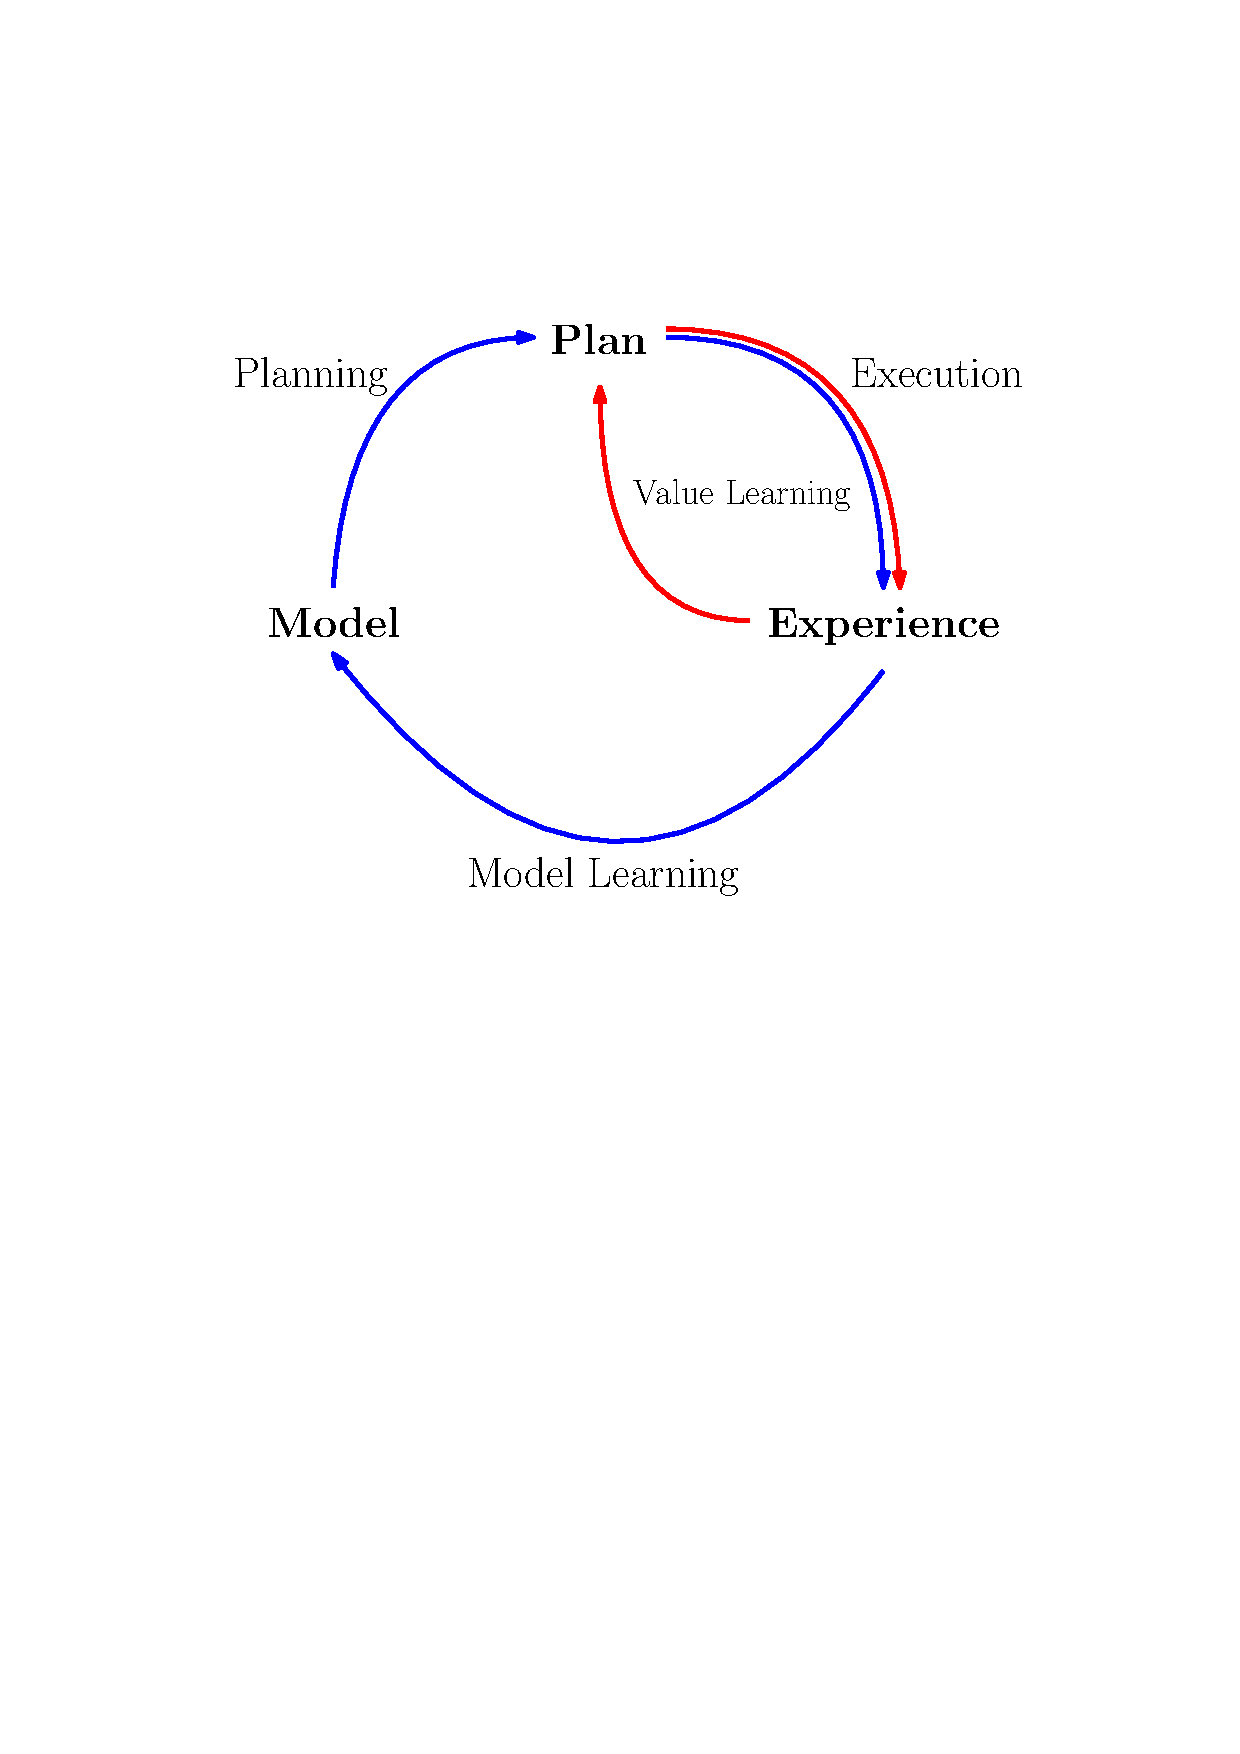
\includegraphics[width=0.5\linewidth]{figures/intro/dyna.pdf}
  \caption{Operation of Model-based (blue) and Model-Free RL (red) methods
    while executing in unknown environments and collecting
    experience to complete a task. Figure inspired from Dyna~\cite{DBLP:journals/sigart/Sutton91}}
  \label{fig:dyna}
\end{figure}

\subsection{Updating the Behavior of the Planner}
\label{sec:updat-behav-plann}


In contrast, the latter direction of updating the behavior of the
planner using online experience has not been explored as extensively
in past literature. Interestingly, this direction has been in use by
the practitioner for quite some time. As motivated earlier, in most
robotic tasks we seldom have access to accurate dynamical models and
the models we use for planning are often inaccurate. Robotics
engineers and practitioners have been dealing with these inaccuracies
by modifying how the planner uses the inaccurate model rather than
updating the model to improve its accuracy. As an example, consider
the task of planning footsteps of a mobile quadruped robot over
partially unknown terrain as shown in Figure~\ref{fig:zucker} taken
from \cite{DBLP:journals/ijrr/ZuckerRSCBAK11}. The
unknown part of the terrain is annotated in the figure (red oval.) To
ensure that the planner does not compute footstep trajectory that goes
through this region, a simple
hack that the practitioner does is to inflate the cost of any
state-action pair that takes the robot into this region. This results
in biasing the planner away from this region thereby updating its
behavior. There are several other works that deal with inaccurate modeling by simply updating the
behavior of the planner~\cite{DBLP:journals/ral/McConachiePMB20,
  DBLP:journals/scirobotics/MitranoMB21, DBLP:journals/ral/PowerB21,
  DBLP:conf/icra/LeeFTRGRF20}.

An observant reader will notice that these approaches require the models used
for planning to not be completely inaccurate everywhere. As a simple example, if
we use a model that predicts that the robot will crash for any action that it
can possibly take, then simply updating the behavior of the planner will not
result in any improvement as the model used is inherently bad.
While these
approaches have been explored in practice, there is very little prior work that has studied this
direction from a theoretical point of view aiming to understand the
assumptions required to guarantee task completeness, and a systematic
study to analyze its empirical performance in practice. This thesis
aims to fill this gap and develop a better understanding when, where,
and how these methods work well in practice.

\section{Thesis Goal and Contributions}
\label{sec:thes-goal-contr}

While most existing works have presented and studied approaches that
use the experience from executions to update the dynamics of the
inaccurate model, one can argue that this is wasteful if we are interested in
completing the task and not in modeling the dynamics
accurately. Furthermore, robots operating in the real world have
operating constraints that require them to quickly adapt to
new scenarios and not spend hours acquiring experience to learn true
dynamics. Finally in tasks where the dynamics are complicated, it could be
computationally infeasible to have a representation in the model class that can
capture the true dynamics. In light of these challenges and insights, the goal
of this thesis is to justify the following statement:

\begin{quote}
\textit{By updating the
behavior of the planner and not the dynamics of the model, we can
leverage simplified and potentially inaccurate models and
significantly reduce the amount of real-world experience needed to
provably guarantee that the robot completes the task.}
\end{quote}

\begin{figure}[t]
  \centering
  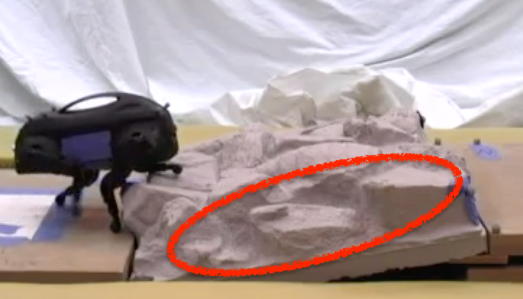
\includegraphics[width=0.5\linewidth]{figures/intro/zucker}
  \caption{A practitioner's approach to dealing with inaccuracies in
    dynamical models used for planning. In this example, the robot is
    planning a footstep trajectory along the partially unknown terrain
  to reach the other side. The planner has access to a model of the
  terrain which is inaccurate in the regions marked by red oval. To
  ensure that the planner does not compute any trajectory going
  through the red oval region, practitioners typically inflate the
  cost of any action executed within the region or any action that
  takes the robot into this region. This results in biasing the
  planner away from this region thereby updating its behavior. Figure
  taken from \cite{DBLP:journals/ijrr/ZuckerRSCBAK11} and the red oval
  region depicted is an example used for emphasis.}
\label{fig:zucker}
\end{figure}

% We support this argument by presenting two methods that update the
% behavior of the planner and do not require any updates to the dynamics
% of the inaccurate model used for planning.  Both methods come with
% provable guarantees on completing the task under some assumptions on the
% accuracy of the model. In addition to these methods, we also emphasize
% the importance of using model-based methods
% by analyzing the sample complexity (or the amount of experience
% needed) of exploration techniques used in model-free RL methods. Our
% analysis shows that undirected global exploration techniques popularly
% used in model-free RL methods can result in large sample complexity
% requirements that cannot be realized in practice on a robot. Furthermore to understand the
% effectiveness of using a potentially inaccurate model, we consider the linear
% quadratic control problem with unknown transition dynamics and show that the
% worst case performance that can be achieved is bounded even with significant
% modeling errors.

We support this argument through the primary contributions of this thesis which
are detailed in the following sections.

%The primary contributions of this thesis can be detailed as follows.

\subsection{Sample Complexity of Exploration in Model-Free Policy
  Search}
\label{sec:sample-compl-expl}
We analyze the sample complexity of exploration techniques in
  model-free RL methods. This analysis is presented by viewing model-free policy
  search methods through the lens of derivative-free optimization (DFO)
  and computing worst case upper bounds on the number of samples
  required to compute a $\epsilon$-suboptimal policy. We present a DFO
  point of view for methods that involve either exploration in action
  space or exploration in policy space, and present trade-offs between
  both styles of exploration in terms of the dimensionality of the
  policy parameter space, and the horizon length of the task. This
  analysis is presented in Chapter~\ref{CHA:ARS} of the
  thesis and is also presented in our paper~\cite{aistats19}. In addition
  to contrasting exploration in policy space vs action space, this
  work also emphasizes the large sample complexity required by
  model-free methods, which cannot be realized in practice on a robot.
  
\subsection{Planning and Execution using Inaccurate Models}
\label{sec:plann-exec-using}
  We present the first systematic effort to understand methods
  that use online experience from executions to update the behavior of
  the planner and not update the dynamics of the model. These
  methods can make progress towards completing the task despite using
  a potentially inaccurate model. One can construct cases where if the
  model is highly inaccurate (e.g. a model that predicts a humanoid
  falling down for any action and failing to complete the task of
  moving forward,) then such a method cannot be expected to finish the
  task. Hence, we study the assumptions required on the accuracy of
  the model used for planning that ensures task completeness without
  requiring any updates to the dynamics of the model. Furthermore, we
  frame our problem in the purely online setting where the experience
  gathered by the robot is along a single trajectory without any
  access to resets. We believe that this setting is realistic and has
  challenges that these methods are uniquely positioned to tackle.

  We propose \cmax{}, an approach that guarantees that the robot
  completes the task using the inaccurate model without any resets and
  without requiring any updates to the dynamics of the model. This is
  achieved by biasing the planner away from transitions whose dynamics
  are discovered to be inaccurately modeled during online
  execution. On the theoretical side, we establish provable guarantees
  on task completeness under assumptions on the accuracy of the model
  used for planning. Empirically, we show that \cmax{} outperforms
  state-of-the-art model-free and model-based RL methods in terms of
  the number of executions taken to complete the task. Crucially,
  \cmax{} exhibits goal-driven behavior which enables it to focus on
  completing the task as quickly as possible and not waste executions  
  learning the true dynamics. This method is explained in detail in
  Chapter~\ref{CHA:CMAX} and is also presented in our
  paper~\cite{cmax}.

\subsection{Leveraging Experience in Planning and Execution using
  Inaccurate Models}
\label{sec:lever-exper-plann}
  
While a robot using \cmax{} is provably guaranteed to complete
  the task, it requires strong assumptions on the accuracy of the
  model that are often not realized in practice and hard to verify
  prior to execution. Furthermore for repetitive tasks, \cmax{} fails
  to improve the quality of the solution over repetitions of the same
  task as it does not leverage previously discovered inaccurately
  modeled transitions. This is remedied by our second approach
  \cmaxpp{} that leverages experience from past executions to improve
  the quality of solution over repetitions of the same
  task. Crucially unlike \cmax{}, \cmaxpp{} can compute solution
  plans that contain previously discovered inaccurately modeled
  transitions. \cmaxpp{} achieves this by integrating model-free value
  learning using acquired experience with model-based planning using
  the inaccurate model. As a consequence of this in addition to
  completeness, \cmaxpp{} also guarantees asymptotic convergence to
  the optimal path cost as the number of repetitions increases. These
  guarantees of \cmaxpp{} are established under assumptions on the
  accuracy of the model that are much more relaxed compared to the
  assumptions required by \cmax{}. Importantly, like \cmax{},
  \cmaxpp{} never updates the dynamics of the model. This method is
  explained in detail in Chapter~\ref{CHA:CMAXPP} and is also
  presented in our paper~\cite{cmaxpp}.

\subsection{On the Effectiveness of Using Inaccurate Models}
\label{sec:effect-using-inacc}

In Chapters~\ref{CHA:CMAX} and~\ref{CHA:CMAXPP}, the focus is on proving task
completeness guarantees for methods that update the behavior of the planner.
However, there are no provable guarantees on the performance of the plan as a
function of the modeling error. This is especially useful in understanding how
accurate a model needs to be, in order to converge to a plan that has bounded
worst case performance. To derive such a guarantee, we study the control of
linearized systems with quadratic costs which is easier to analyze and provides insights
into the performance we can expect from using an inaccurate model. In this
setting, we analyze the performance of \textit{iterative learning control} (ILC)
approaches that use online experience from executions to update the behavior of
the planner and do not update the model, similar to \cmax{} and \cmaxpp{}. We
present upper bounds in terms of modeling error on the sub-optimality gap between the cost incurred by the
controller that ILC converges to, and the cost incurred by using the optimal
linear quadratic controller. Our analysis shows that the sub-optimality gap
bound for ILC has a nice quadratic dependency on the modeling error. Furthermore, our
analysis also highlights the
pitfalls of methods that naively use inaccurate models without updating the
behavior of the planner. For these methods, the sub-optimality gap bound has a
dependence on quadratic and higher-order terms in modeling error that can make it
significantly worse than ILC when modeling error is significant. This analysis
is explained in detail in Chapter~\ref{CHA:ILC} and is also presented in our
paper~\cite{ilc}.

\subsection{Task-Aware Online Model Search with Misspecified Model Classes}
\label{sec:task-aware-model}

Our final contribution departs from the algorithms developed so far, and studies
the alternative of using experience from executions to update the dynamics of
the model. More precisely, we study the problem of planning in an environment
with unknown transition dynamics when given access to a misspecified model
class. A model class is misspecified if no model in the class can capture the
true dynamics of the environment, which is usually the case in real-world
domains where we either have limited domain knowledge or we would like to use a
small model for computational efficiency. In such a setting, finding a model
that optimizes prediction error, as done in most of the existing work, can
lead to poor task performance when the model is used for planning. We develop a
model learning method \taml{} that is task-aware, i.e. optimizes completing the task
when used for planning, rather than prediction error. We achieve this
by performing derivative-free optimization in the space of model
parameters to explicitly select a model that 
results in a policy, upon planning, that achieves the best task performance
during execution. To measure the performance of any policy in the
environment without executing it, we rely on a monte-carlo evaluation procedure
that uses the experience accumulated so far in
state-action regions where we have good coverage, and fall back on an
optimistic model everywhere else. Theoretically, we can show that given
unlimited computation, \taml{} is guaranteed to reach the goal in
small state-action spaces as long as there is at least one good
performing model in the model class. Empirically, we show that \taml{} performs
significantly better than traditional model learning methods that optimize
prediction error in a simple mountain car domain. This work is explained in
detail in Chapter~\ref{CHA:TAML}.

\section{Bibliographical Remarks}
\label{sec:bibl-remarks}

This thesis only contains works for which this author is the primary
contributor.

Chapter~\ref{CHA:ARS} is based on joint work with Wen Sun and Drew Bagnell
that appeared in~\cite{aistats19}.
Chapter~\ref{CHA:CMAX} is based on joint work with Yash Oza, Drew Bagnell, and Max
Likhachev that appeared in~\cite{cmax}.
Chapter~\ref{CHA:CMAXPP} is based on joint work with Drew Bagnell and Max
Likhachev that appeared in~\cite{cmaxpp}.
Chapter~\ref{CHA:ILC} is based on joint work with Wen Sun, Max Likhachev,
and Drew Bagnell that appeared in~\cite{ilc}.
Chapter~\ref{CHA:TAML} is based on ongoing work with Sanjiban Choudhury, Drew
Bagnell, and Max Likhachev.

\section{Open Source Software}
\label{sec:open-source-software}

The author is a huge proponent of open sourcing research
code. Previously open sourced code has hugely benefitted the work in
this thesis, and the author would like to give back to the community
by open sourcing all the code for this thesis. The links to code are
listed below:
\begin{enumerate}
\item Chapter~\ref{CHA:ARS} code can be found at
  \url{https://github.com/LAIRLAB/contrasting_exploration_rl}
\item Chapter~\ref{CHA:CMAX} code can be found at
  \url{https://github.com/vvanirudh/CMAX}
\item Chapter~\ref{CHA:CMAXPP} code can be found at
  \url{https://github.com/vvanirudh/CMAXPP}
\item Chapter~\ref{CHA:ILC} code can be found at
  \url{https://github.com/vvanirudh/ILC.jl}
\item Chapter~\ref{CHA:TAML} code can be found at
  \url{https://github.com/vvanirudh/TOMS.jl}
\end{enumerate}

\section{Excluded Research}
\label{sec:excluded-research}

The author has excluded a significant portion of his doctoral work for the
purpose of keeping this thesis succinct. The excluded works are listed below:
\begin{enumerate}
  \item TRON: A Fast Solver for Trajectory Optimization with Non-Smooth Cost
        Functions, that appeared in~\cite{tron}.
  \item Planning, Learning and Reasoning Framework for Robot Truck Unloading,
        that appeared in~\cite{truck}.
  \item Provably Efficient Imitation Learning from Observation Alone, that
        appeared in \cite{fail}.
  \item Improved Soft Duplicate Detection in Search-Based Motion Planning, that
        appeared in~\cite{duplicate}.
  \item Task-informed Fidelity Management for Speeding up Robotics Simulation,
        that appeared in~\cite{fidelity}.
\end{enumerate}


%%% Local Variables:
%%% mode: latex
%%% TeX-master: "../main"
%%% End:
